\documentclass[a4paper,10pt]{article}
% Språk och encodings
\usepackage[swedish,english]{babel}
\usepackage[T1]{fontenc}
\usepackage[utf8]{inputenc}
\usepackage[fixlanguage]{babelbib}
% Images and floats
\usepackage{graphicx}
\usepackage{wrapfig}
\usepackage{float}
% Clear type + Sans-serif font
\usepackage{lmodern}
\renewcommand{\familydefault}{\sfdefault}
% Avancerade tabeller
\usepackage{tabularx}
\usepackage{multirow}
\usepackage{booktabs}
% Matte
\usepackage{amsmath, amsthm, amssymb}
% Algoritmer
\usepackage[ruled,vlined]{algorithm2e}
% Källkod
\usepackage{listings}
\lstset{
	showspaces = false,
	showstringspaces = false,
}
% Inkludera pdf-sidor
\usepackage{pdfpages}
% Länkar
\usepackage{color}
\definecolor{dark-blue}{rgb}{0, 0, 0.6}
\usepackage{hyperref}
\hypersetup{
  colorlinks=true,
  linkcolor=dark-blue,
  urlcolor=dark-blue
}
% Vettiga paragrafer
\setlength{\parindent}{0pt}
\setlength{\parskip}{2ex}

% Kommando för kommandorader
\newcommand{\cmdline}[1]{\mbox{\textbf{\texttt{> #1}}}}

% Sidhuvud/sidfot
\usepackage{fancyhdr}
\setlength{\headheight}{15pt}
\pagestyle{fancyplain}
\lfoot{Carl-Oscar Erneholm \\ 880422-0872 \\ coer@kth.se}
\rfoot{Martin Nycander \\ 881028-0076 \\ mnyc@kth.se}
\cfoot{Page \thepage}

% Språk
\selectbiblanguage{swedish}
\selectlanguage{swedish}

% Titel
\title{Laborationsrapport 1 \\ Digenv - processkommunikation med pipes v1.1}
\author{Carl-Oscar Erneholm \and Martin Nycander}
\date{\today}

\begin{document}

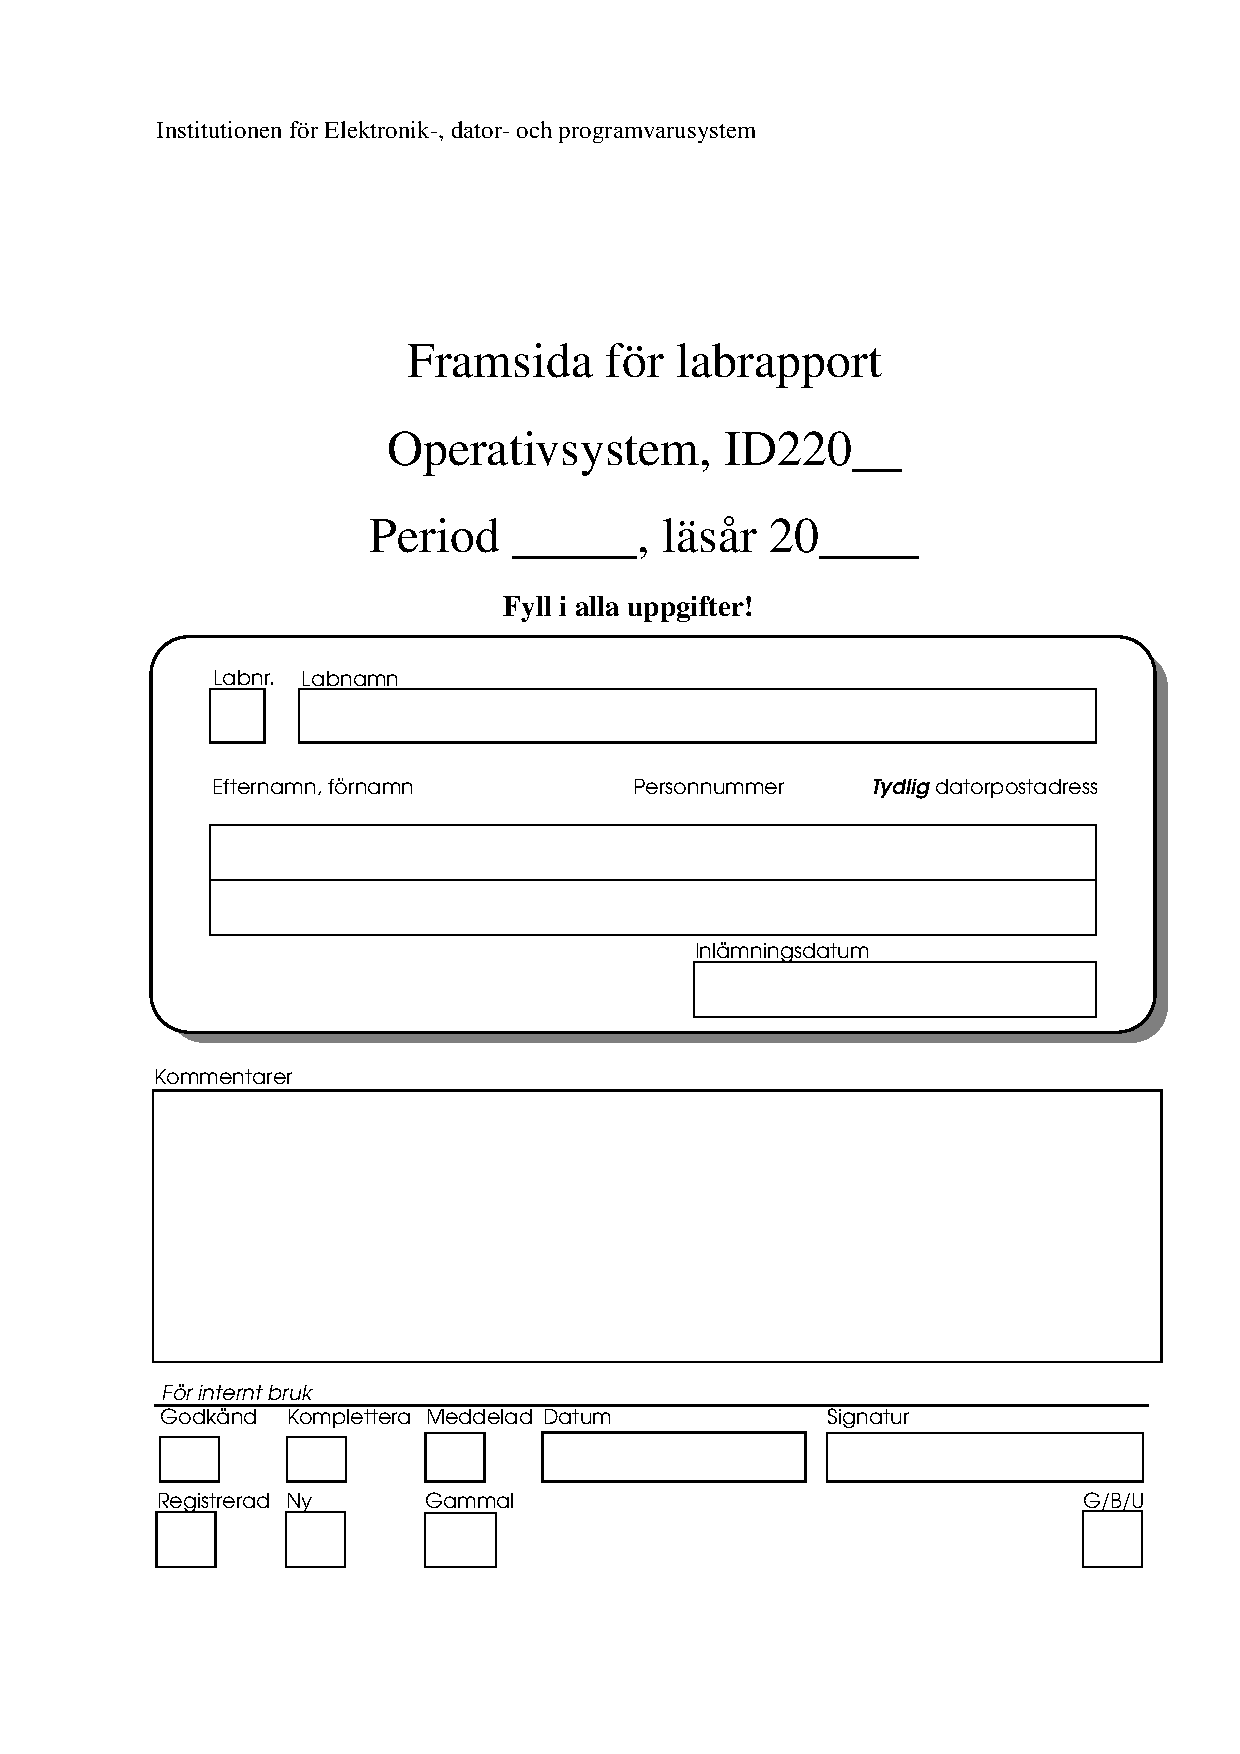
\includepdf[pages=-]{framsida.pdf}

\maketitle

\section{Problembeskivning}

Uppgiften handlar om att skriva ett litet program som körs på följande vis: \\
\cmdline{digenv [parameterlista]} \\
Körs programmet utan parametrar ska det vara ekvivalent med att köra: \\
\cmdline{printenv | sort | less} \\
Där ``less'' ersätts med vad än som står i environmentvariabeln \verb!PAGER!. Om inte \verb!PAGER! är satt används \verb!less!; och om inte \verb!less! finns så används \verb!more!.

Körs programmet med parametrar så ska följande köras: \\
\cmdline{printenv | grep parameterlista | sort | less} \\
Samma regler för ``less'' gäller här.

Det är inte tillåtet att använda C-bibliotekets funktion \verb!system(3)!.

\subsection{Förberedelsefrågor}


\begin{enumerate}
	\item[1.] \textbf{\footnotesize När en maskin bootar med UNIX skapas en process som har PID=1 och den lever så länge maskinen är uppe. Från den här processen skapas alla andra processer med fork. Vad heter denna process?}
	
	Processen som skapas först heter \verb!init!.

	\item[2.] \textbf{\footnotesize Kan environmentvariabler användas för att kommunicera mellan föräldra- och barnprocess? Åt bägge hållen?}

	Environmentvariabler kan användas för att kommunicera mellan föräldra- och barnprocesser eftersom dom i praktiken är globala variabler i systemet. Vi ser inga problem med att kommunikation sker åt båda hållen.

	\item[3.] \textbf{\footnotesize Man kan tänka sig att skapa en odödlig child-process som fångar alla SIGKILL-signaler genom att registrera en egen signalhanterare kill\_handler som bara struntar i SIGKILL. Processen ska förstås ligga i en oändlig loop då den inte exekverar signalhanteraren. Testa! Skriv ett programmet med en sådan signalhanterare, kompilera och provkör. Vad händer? Läs mer i manualtexten om sigaction för att förklara resultatet.}

	Man kan fånga alla signaler förutom \verb!SIGKILL! och \verb!SIGSTOP!. Men andra ord går det inte att skapa en odödlig process. Empiriska tester har även visat detta.

	\item[4.] \textbf{\footnotesize Varför returnerar fork 0 till child-processen och child-PID till parent-processen, i stället för tvärtom?}

	\verb!fork! returnerar 0 till child-processen och \verb!child-PID! till parent-processen eftersom det är föräldern måste kunna identifiera de olika barnen för att kontrollera eventuella returvärden. Barn-processer bör dock inte ta någon kontroll över föräldern.

	\item[5.] \textbf{\footnotesize UNIX håller flera nivåer av tabeller för öppna filer, både en användarspecifik ``File Descriptor Table'' och en global ``File Table''. Behövs egentligen File Table? Kan man ha offset i File Descriptor Table istället?}

	File table behövs om andra processer ska kunna ta reda på vilka andra processer som har öppnat filen. Om detta inte är ett krav går det jättebra att göra en enda stor tabell, man måste dock tillåta flera radera i tabellen per fil (inga krav på unika värden).

	\item[6.] \textbf{\footnotesize Kan man strunta i att stänga en pipe om man inte använder den? Hur skulle programbeteendet påverkas? Testa själv. Läs mer i pipe(2).}

	Om man inte stänger skrivdelen av \verb!pipe!:en till barnprocessen så kommer den aldrig få \verb!EOF! och troligtvis aldrig returnera. Praxis bör vara att alltid stänga den delen av \verb!pipe!:en som man inte ska använda först.

	Programmet kommer antagligen hamna i deadlock om man glömmer stänga en \verb!pipe!.

	\item[7.] \textbf{\footnotesize Vad händer om en av processerna plötsligt dör? Kan den andra processen upptäcka detta?}

	Om den andra processen har en pipe öppen så kommer den när den läser från \verb!pipe!:en att få signalen \verb!SIGPIPE! från kerneln, vilket meddelar att den andra processen har dött. Om man inte skrivit en signal handler så kommer programmet att terminera.

	\item[8.] \textbf{\footnotesize Hur kan du i ditt program ta reda på om grep misslyckades? Dvs om grep inte hittade någon förekomst av det den skulle söka efter eller om du gett felaktiga parametrar till grep?}

	Vårt program kan undersöka \verb!grep!:s returvärde. Den kommer returnera 0 om allt gick bra, 1 om den inte hittade någon rad, och 2 om något var fel.	
\end{enumerate}

\section{Programbeskrivning}

\newpage
\section{Tester}

För att testa funktionaliten av vårat program har vi valt att köra följande kontrollerade tester:

\begin{table}[H]
	% PAGER satt
	\begin{tabularx}{\textwidth}{>{\bfseries}r  X }
		\multicolumn{2}{c}{\large\textbf{Testfall 1}} \\[0.1cm]
		\toprule	Beskrivning				& Inläsning av PAGER-variabeln \\
		\midrule	Förkrav					& Miljövariabeln \texttt{PAGER} är satt till ``pg''. \\
		\midrule	Körning					& \cmdline{./digenv} \\
		\midrule	Förväntat resultat		& Programmet ``pg'' startas med godtyckligt innehåll. \\
		\bottomrule
	\end{tabularx}
\end{table}

\begin{table}[H]
	% PAGER inte satt (med less)
	\begin{tabularx}{\textwidth}{>{\bfseries}r  X }
		\multicolumn{2}{c}{\large\textbf{Testfall 2}} \\[0.1cm]
		\toprule	Beskrivning				& Misslyckad inläsning av PAGER-variabeln \\
		\midrule	Förkrav					& Miljövariabeln \texttt{PAGER} finns inte, programmet ``less'' finns i path:en. \\
		\midrule	Körning					& \cmdline{./digenv} \\
		\midrule	Förväntat resultat		& Programmet ``less'' startas med godtyckligt innehåll. \\
		\bottomrule
	\end{tabularx}
\end{table}

\begin{table}[H]
	% PAGER inte satt (utan less)
	\begin{tabularx}{\textwidth}{>{\bfseries}r  X }
		\multicolumn{2}{c}{\large\textbf{Testfall 3}} \\[0.1cm]
		\toprule	Beskrivning				& Misslyckad inläsning av PAGER-variabeln, utan ``less'' \\
		\midrule	Förkrav					& Miljövariabeln \texttt{PAGER} finns inte, programmet ``less'' finns inte i path:en. Programmet ``more'' finns i path:en. \\
		\midrule	Körning					& \cmdline{./digenv} \\
		\midrule	Förväntat resultat		& Programmet ``more'' startas med godtyckligt innehåll. \\
		\bottomrule
	\end{tabularx}
\end{table}

\begin{table}[H]
	\begin{tabularx}{\textwidth}{>{\bfseries}r  X }
		\multicolumn{2}{c}{\large\textbf{Testfall 4}} \\[0.1cm]
		\toprule	Beskrivning				& Normal användning med filtrering \\
		\midrule	Förkrav					& Miljövariabeln \texttt{PAGER} är satt till ``less''. \\
		\midrule	Körning					& \cmdline{./digenv PATH} \\
		\midrule	Förväntat resultat		& \begin{itemize}
  			\setlength{\itemsep}{0pt}
  			\setlength{\parskip}{0pt}
  			\setlength{\parsep}{0pt}
			\item Utskrift och tillstånd ska vara ekvivalent med: \cmdline{printenv | grep PATH | sort | less}
			\item Inga oavslutade barn-procceser finns. Verifiera med \cmdline{ps -ef}.
			\item Inga temporära datafiler har skapats.
		\end{itemize} \\
		\bottomrule
	\end{tabularx}
\end{table}

\begin{table}[H]
	\begin{tabularx}{\textwidth}{>{\bfseries}r  X }
		\multicolumn{2}{c}{\large\textbf{Testfall 5}} \\[0.1cm]
		\toprule	Beskrivning				& Normal användning med filtrering och flaggor \\
		\midrule	Förkrav					& Miljövariabeln \texttt{PAGER} är satt till ``less''. \\
		\midrule	Körning					& \cmdline{./digenv -i pAtH} \\
		\midrule	Förväntat resultat		& Samma som testfall 3. \\
		\bottomrule
	\end{tabularx}
\end{table}

\begin{table}[H]
	\begin{tabularx}{\textwidth}{>{\bfseries}r  X }
		\multicolumn{2}{c}{\large\textbf{Testfall 6}} \\[0.1cm]
		\toprule	Beskrivning				& Syntaxfel i argument till grep \\
		\midrule	Förkrav					& - \\
		\midrule	Körning					& \cmdline{./digenv -.} \\
		\midrule	Förväntat resultat		& \begin{itemize}
  			\setlength{\itemsep}{0pt}
  			\setlength{\parskip}{0pt}
  			\setlength{\parsep}{0pt}
			\item Programmet avbryts.
			\item Ett felmeddelande kan skrivas till \texttt{stderr}.
			\item Resultatet av ``\cmdline{echo \$?}'' ska inte bli $0$.
			\item Inga oavslutade barn-procceser finns. Verifiera med \cmdline{ps -ef}.
			\item Inga temporära datafiler har skapats.
		\end{itemize} \\
		\bottomrule
	\end{tabularx}
\end{table}

\section{Resultat}

Körning av ovanstående standardiserade testfall gav följande resultat.

\begin{tabularx}{\textwidth}{>{\bfseries}l  X }
	\multicolumn{2}{c}{\large\textbf{Testfallsresultat}} \\[0.1cm]
	\toprule
	1. Inläsning av PAGER-variabeln 							& Godkänd \\
	2. Misslyckad inläsning av PAGER-variabeln					& Godkänd \\
	3. Misslyckad inläsning av PAGER-variabeln, utan ``less''	& Godkänd \\
	4. Normal användning med filtrering 						& Godkänd \\
	5. Normal användning med filtrering och flaggor				& Godkänd \\
	6. Syntaxfel i argument till grep							& Godkänd \\
	\bottomrule
\end{tabularx}

\subsection{Exempelutskrift från testfall 4}

\lstset{breaklines=true}
\begin{lstlisting}
u3:~/kurser/os11>./digenv 
GROUP=dip
HOME=/afs/nada.kth.se/home/x/u1hbudlx
HOSTTYPE=x86_64-linux
HOST=u3.csc.kth.se
INFOPATH=/usr/local/hacks/info/
KRB5CCNAME=FILE:/tmp/krb5cc_43056_s28404
LANG=en_US.UTF-8
_LMFILES_=/afs/nada.kth.se/common/usr/local/lib/module/modules/hacks/z:/afs/nada.kth.se/common/usr/local/lib/module/modules/sima/user:/afs/nada.kth.se/common/usr/local/lib/module/modules/tex/3.0:/afs/nada.kth.se/common/usr/local/lib/module/modules/sfw/Linux:/afs/nada.kth.se/common/usr/local/lib/module/modules/gcc/4.0.2:/afs/nada.kth.se/common/usr/local/lib/module/modules/pgsql/7.4.16
LOADEDMODULES=hacks/z:sima/user:tex/3.0:sfw/Linux:gcc/4.0.2:pgsql/7.4.16
LOGNAME=mnyc
MACHTYPE=x86_64
MAIL=/var/mail/mnyc
MANPATH=::/usr/local/hacks/man
MODULEPATH=/usr/local/Modules/versions:/usr/local/Modules/$MODULE_VERSION/modulefiles:/afs/nada.kth.se/common/usr/local/lib/module/modules:/usr/local/hacks/common/modules
MODULESHOME=/usr/local/Modules/3.2.7
MODULE_VERSION=3.2.7
MODULE_VERSION_STACK=3.2.7
OSTYPE=linux
PAGER=less
PATH=/pkg/sima/1.0/client:/usr/local/sbin:/usr/local/bin:/usr/sbin:/usr/bin:/sbin:/bin:/usr/games:/usr/local/hacks/bin
PWD=/afs/nada.kth.se/home/x/u1hbudlx/kurser/os11
REMOTEHOST=s213-103-214-88.cust.tele2.se
SHELL=/bin/tcsh
SHLVL=1
SSH_CLIENT=213.103.214.88 12847 22
SSH_CONNECTION=213.103.214.88 12847 130.237.223.91 22
SSH_TTY=/dev/pts/3
TERM=xterm
USER=mnyc
VENDOR=unknown
XAUTHORITY=/tmp/.Xauthority.y28404
XUSERFILESEARCHPATH=/usr/local/hacks/app-defaults/%N
\end{lstlisting}

\subsection{Exempelutskrift från testfall 6}

\begin{lstlisting}
u3:~/kurser/os11>./digenv -.
grep: invalid option -- '.'
Usage: grep [OPTION]... PATTERN [FILE]...
Try `grep --help' for more information.
u3:~/kurser/os11>
\end{lstlisting}

\section{Labbutvärdering}

Ungefärlig nedlagd tid på labben: $1 \text{ heltidsvecka} \cdot 2 \text{ personer}$.

Ett labPM borde enbart kortfattat och strikt formulera uppgiften och vilka krav som finns.
Eventuell hjälpinformation borde finnas i separat bilaga. Att ha allt i ett enda häfte är väldigt rörigt och gör att det tar väldigt lång tid att sätta sig in i alla aspekter av området som ska laboreras kring.

Förutom lite förståelse kring hur pipes fungerar på en lägre nivå så känner vi inte att laborationen har gett så mycket ny kunskap. Förberedelseuppgifterna stod för den större delen av insikter och inlärning. Programmeringsspråket C har vi harvat med förut; och precis som tidigare bråkade vi mest med språket och inte med teorin.

På en skala 1-5 ger vi den $2$. Själva labben kan förbättras med fler förberedelsefrågor och deluppgifter, exempelvis att man först skriver ett program där \verb!fork! testas, ett där de olika varianterna av \verb!exec! testas och de lite utvärdering över hur man kan läsa ut returvärden. Avsaknad av ``delinlämningar'' kan orsaka håravfall, koffeinförgiftning, panik, ångest, panikångest, övernattningar i laborationssalar och ett starkt hat för ansi c (en 20 år gammal standard -- ursäkta?).


\end{document}